\chapter{Instruments d'optique et œil}\label{ch:b1:optical-instruments}

Du dernier rang d'une salle de concert, une paire de jumelles ramène le
visage de la chanteuse à portée de bras~; un \omterm{def:b1:optical-instruments:microscope}{microscope} transforme une
goutte d'eau d'étang en ménagerie~; un téléphone épais comme un doigt
photographie la Voie lactée. Chacun de ces instruments n'est qu'un
petit nombre de \omterm{def:b1:mirrors-thin-lenses:lens}{lentilles minces} disposées dans un seul but~: présenter
à l'\omterm{def:b1:optical-instruments:eye}{œil}, ou à un capteur, une image plus grande, plus lumineuse ou plus
fine que celle que l'\omterm{def:b1:optical-instruments:eye}{œil} formerait seul. Ce chapitre commence donc par
l'\omterm{def:b1:optical-instruments:eye}{œil} lui-même --- ce qu'il peut et ce qu'il ne peut pas --- puis
construit la \omterm{def:b1:optical-instruments:G}{loupe}, le \omterm{def:b1:optical-instruments:microscope}{microscope}, la lunette et l'\omterm{def:b1:optical-instruments:camera}{appareil
photographique} à partir de la relation de conjugaison du chapitre
précédent.

\begin{omfigure}
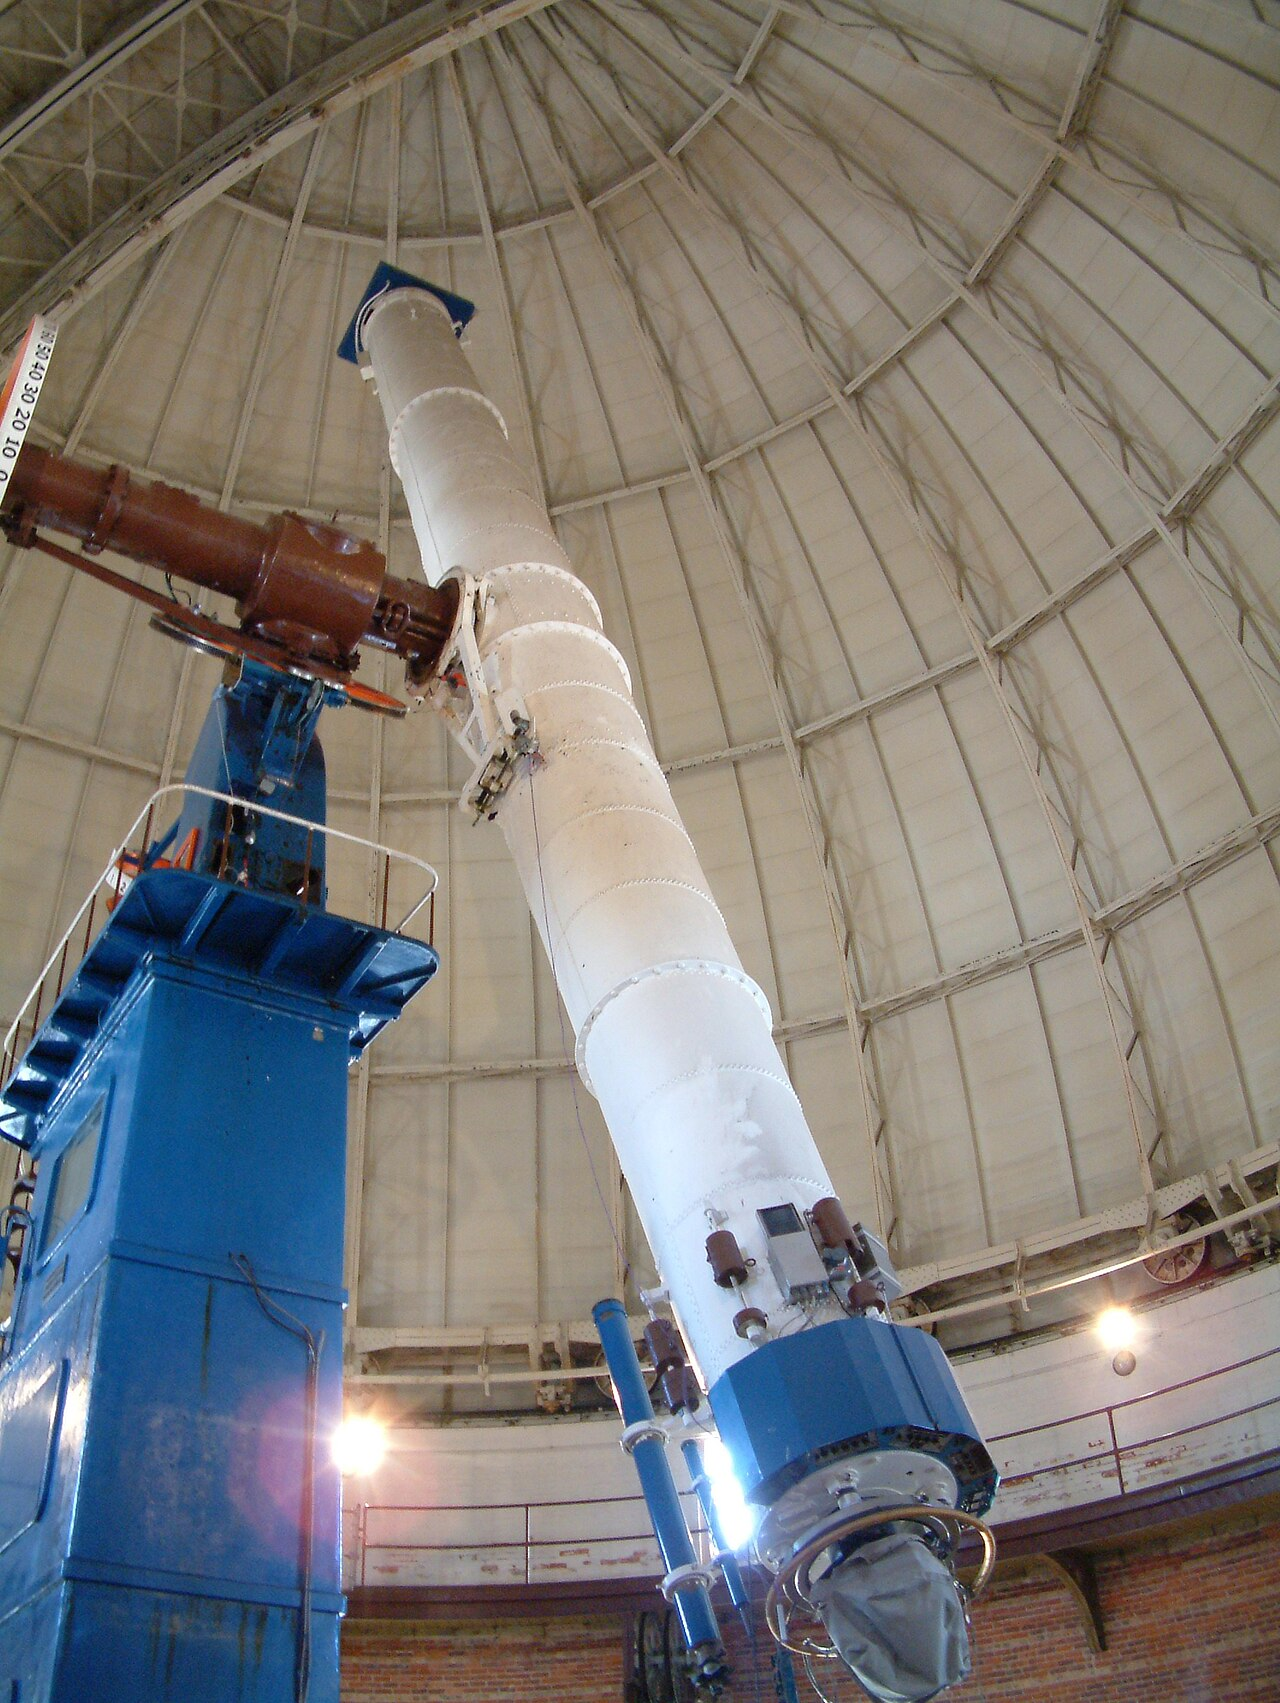
\includegraphics[width=0.42\linewidth]{images/book3/yerkes-refractor.jpg}

{\small La lunette de 40 pouces de l'observatoire Yerkes (1897), toujours la plus grande lunette jamais construite~: un \omterm{def:b1:optical-instruments:microscope}{objectif} d'un mètre et un tube de dix-neuf. Au-delà de cette taille, une \omterm{def:b1:mirrors-thin-lenses:lens}{lentille} fléchit sous son propre poids, et l'astronomie s'est tournée vers les miroirs.}
\end{omfigure}

\begin{omfigure}
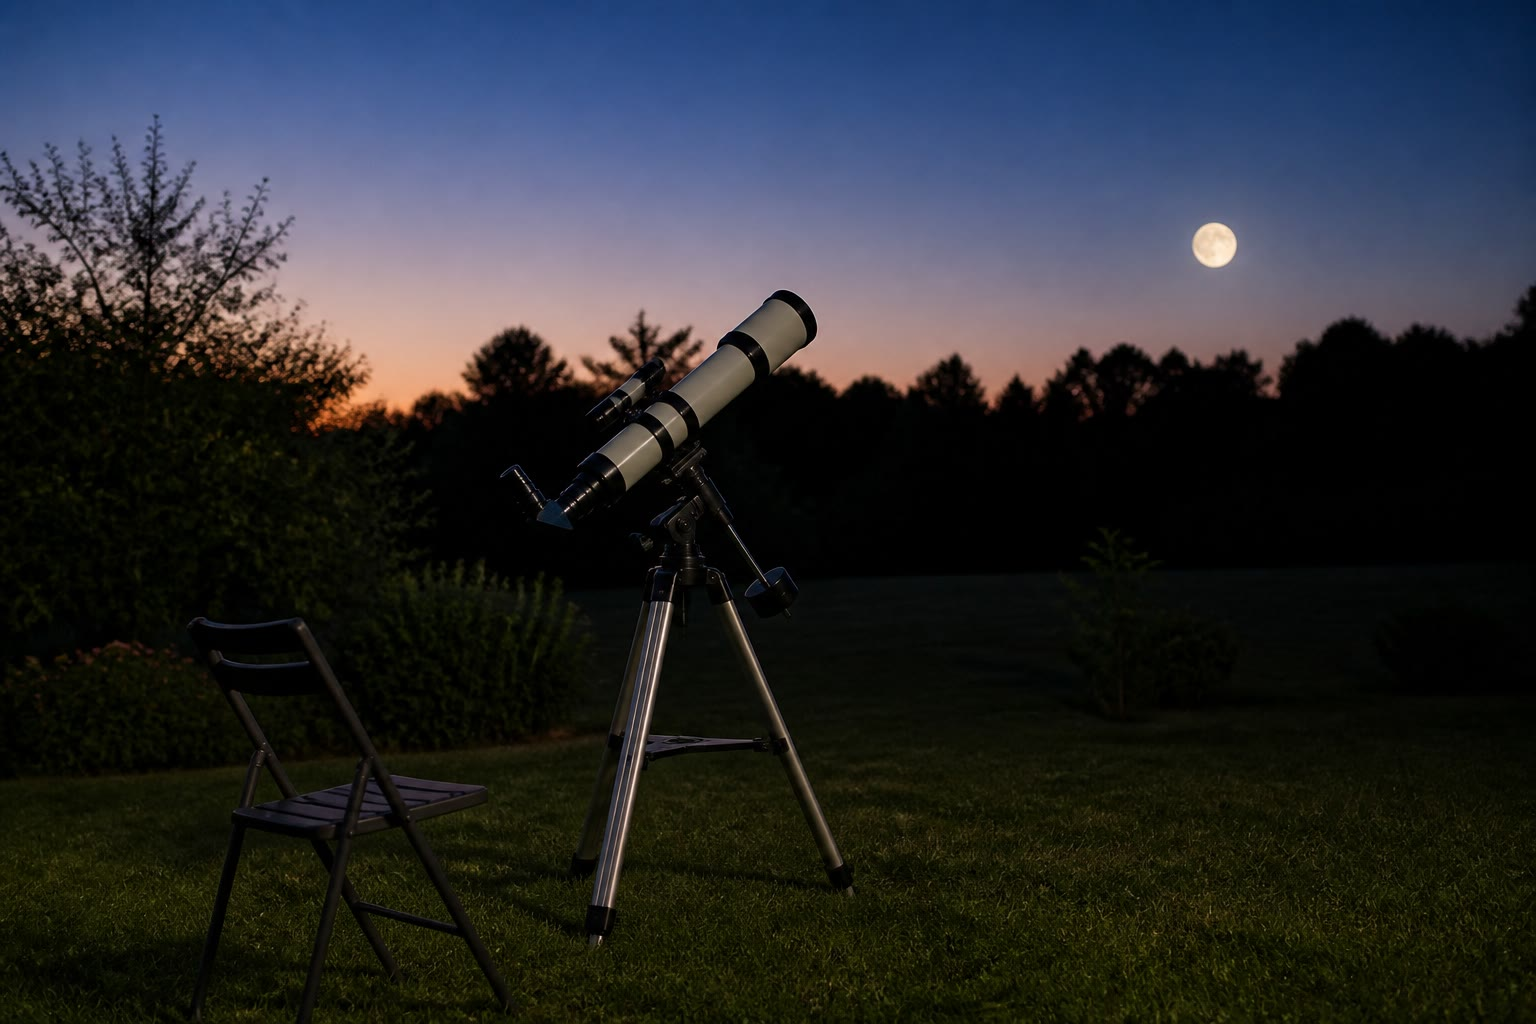
\includegraphics[width=0.58\linewidth]{images/book3/ai/b3-04-telescope-dusk.jpg}

{\small Une petite lunette au crépuscule~: un \omterm{def:b1:optical-instruments:microscope}{objectif} de grande \omterm{def:b1:mirrors-thin-lenses:lens}{distance focale} et un \omterm{def:b1:optical-instruments:microscope}{oculaire} de courte --- la lunette afocale de ce chapitre, pointée vers la Lune de son problème du week-end.}
\end{omfigure}

\section{L'œil}

\begin{definition}[Œil réduit]\label{def:b1:optical-instruments:eye}
\index{œil}\index{œil réduit}\index{rétine}\index{accommodation}
L'\emph{œil réduit} modélise la cornée et le cristallin par une seule
\omterm{def:b1:mirrors-thin-lenses:lens}{lentille mince} convergente de \omterm{def:b1:mirrors-thin-lenses:lens}{distance focale} \emph{variable}, et la
\emph{rétine} par un écran situé à une distance fixe
$d \approx \qty{17}{mm}$ derrière elle. Des muscles changent la courbure
du cristallin pour maintenir sur la rétine l'image de l'objet
regardé~: c'est l'\emph{accommodation}. L'iris, devant le cristallin,
est un diaphragme de diamètre variable, de \qty{2}{} à \qty{8}{mm}~: la
\emph{pupille}.
\end{definition}

\begin{definition}[Punctum remotum, punctum proximum]\label{def:b1:optical-instruments:punctum}
\index{punctum remotum}\index{punctum proximum}\index{amplitude d'accommodation}
Le \emph{punctum remotum} est le point objet vu net sans accommoder~; le
\emph{punctum proximum} est le point le plus proche vu net avec
l'\omterm{def:b1:optical-instruments:eye}{accommodation} maximale. Pour un \omterm{def:b1:optical-instruments:eye}{œil} normal (emmétrope), le punctum
remotum est à l'infini et le punctum proximum à
$d_m \approx \qty{25}{cm}$, la \emph{distance minimale de vision
distincte} conventionnelle. La différence des \omterm{def:b1:mirrors-thin-lenses:lens}{vergences} nécessaires aux
deux est l'\emph{amplitude d'\omterm{def:b1:optical-instruments:eye}{accommodation}}~: environ \qty{4}{\delta}
chez un jeune adulte, décroissante avec l'âge.
\end{definition}

\begin{example}[La vergence de l'œil]\label{ex:b1:optical-instruments:vergence}
Objet lointain~: une image à $d = \qty{17}{mm}$ signifie $f' = \qty{17}{mm}$,
$V = 1/0.017 = \qty{59}{\delta}$. Objet à \qty{25}{cm}~:
$V = 1/0.017 + 1/0.25 = 59 + 4 = \qty{63}{\delta}$. Quatre dioptries
d'\omterm{def:b1:optical-instruments:eye}{accommodation} sur soixante~: le cristallin n'ajoute que quelques pour
cent au travail de la cornée, mais ces quelques pour cent font toute la
lecture.
\end{example}

\begin{proposition}[Défauts et corrections]\label{prop:b1:optical-instruments:defects}
\index{myopie}\index{hypermétropie}\index{presbytie}
Un \omterm{def:b1:optical-instruments:eye}{œil} \emph{myope} est trop convergent~: son \omterm{def:b1:optical-instruments:punctum}{punctum remotum} est à
distance finie $D_r$~; une \omterm{def:b1:mirrors-thin-lenses:lens}{lentille divergente} de \omterm{def:b1:mirrors-thin-lenses:lens}{distance focale}
$f' = -D_r$ (portée près de l'\omterm{def:b1:optical-instruments:eye}{œil}) image l'infini sur le \omterm{def:b1:optical-instruments:punctum}{punctum
remotum} et rétablit la vision de loin. Un \omterm{def:b1:optical-instruments:eye}{œil} \emph{hypermétrope} n'est
pas assez convergent~: son \omterm{def:b1:optical-instruments:punctum}{punctum remotum} est virtuel (derrière l'\omterm{def:b1:optical-instruments:eye}{œil})
et son \omterm{def:b1:optical-instruments:punctum}{punctum proximum} trop éloigné~; une \omterm{def:b1:mirrors-thin-lenses:lens}{lentille convergente} le
corrige. La \emph{presbytie} est la perte d'\omterm{def:b1:optical-instruments:eye}{accommodation} avec l'âge~:
le \omterm{def:b1:optical-instruments:punctum}{punctum proximum} recule et la lecture exige des \omterm{def:b1:mirrors-thin-lenses:lens}{lentilles
convergentes}, quel que soit le \omterm{def:b1:optical-instruments:punctum}{punctum remotum}.
\end{proposition}

\begin{proof}
Une \omterm{def:b1:mirrors-thin-lenses:lens}{lentille} placée près de l'\omterm{def:b1:optical-instruments:eye}{œil} forme avec lui un système dont l'objet
doit être ce que l'\omterm{def:b1:optical-instruments:eye}{œil} sait voir~: la \omterm{def:b1:mirrors-thin-lenses:lens}{lentille} doit transformer un objet
à l'infini en une \omterm{def:b1:mirrors-thin-lenses:image}{image virtuelle} sur le \omterm{def:b1:optical-instruments:punctum}{punctum remotum},
$\overline{OA'} = -D_r$ pour $\overline{OA} = -\infty$, d'où
$f' = \overline{OA'} = -D_r$. Les autres cas relèvent du même argument
avec les points pertinents.
\end{proof}

\begin{omfigure}
\begin{tikzpicture}[font=\small, x=1cm, y=1cm]
  % eye schematic: lens at x=0, retina at x=2.4 (scaled), object far (parallel rays) and near
  \draw[omDef!30, fill=omDef!8] (1.25,0) ellipse (1.45 and 1.15);
  \draw[very thick, omDef, Stealth-Stealth] (0,-0.8) -- (0,0.8);
  \draw[very thick, omThm] (2.6,-0.55) arc (-25:25:1.3);
  \node[omThm, right] at (2.75,0.9) {rétine};
  \node[omDef, above] at (0,0.85) {lentille};
  % far object: parallel rays -> focus on retina at axis
  \draw[omProp, -Stealth] (-3.2,0.5) -- (0,0.5); \draw[omProp] (0,0.5) -- (2.58,0);
  \draw[omProp, -Stealth] (-3.2,-0.5) -- (0,-0.5); \draw[omProp] (0,-0.5) -- (2.58,0);
  \draw[-Stealth] (-3.4,0) -- (3.3,0);
  \node[omProp, left] at (-3.2,0.5) {objet lointain};
  \draw[Stealth-Stealth] (0,-1.35) -- (2.58,-1.35) node[midway, below] {$d \approx \qty{17}{mm}$};
  % near object at x=-2.4 height 0.6 : with accommodation image at retina: drawn as converging rays from B through O
  \begin{scope}[xshift=7.6cm]
  \draw[omDef!30, fill=omDef!8] (1.25,0) ellipse (1.45 and 1.15);
  \draw[very thick, omDef, Stealth-Stealth] (0,-0.8) -- (0,0.8);
  \draw[very thick, omThm] (2.6,-0.55) arc (-25:25:1.3);
  \draw[-Stealth] (-3.4,0) -- (3.3,0);
  \draw[very thick, omThm, -Stealth] (-2.6,0) -- (-2.6,0.6); \node[above] at (-2.6,0.6) {$B$};
  \draw[omProp] (-2.6,0.6) -- (0,0.6) -- (2.58,-0.6);
  \draw[omProp] (-2.6,0.6) -- (0,0.0) -- (2.58,-0.6);
  \draw[omProp] (-2.6,0.6) -- (0,-0.6) -- (2.58,-0.6);
  \node[omThm, below right] at (2.55,-0.6) {$B'$};
  \node[below] at (-0.4,-1.3) {accommodé~: $f'$ raccourci};
  \end{scope}
\end{tikzpicture}

{\small L'\omterm{def:b1:optical-instruments:eye}{œil réduit}~: une \omterm{def:b1:mirrors-thin-lenses:lens}{lentille mince} de \omterm{def:b1:mirrors-thin-lenses:lens}{distance focale} variable et
une \omterm{def:b1:optical-instruments:eye}{rétine} \qty{17}{mm} derrière elle. Au repos, elle met au point les
objets lointains~; en accommodant, elle raccourcit $f'$ pour amener sur
la \omterm{def:b1:optical-instruments:eye}{rétine} l'image d'un objet proche. L'image est renversée --- le
cerveau la remet à l'endroit.}
\end{omfigure}

\begin{definition}[Diamètre apparent et résolution angulaire]\label{def:b1:optical-instruments:angular}
\index{diamètre apparent}\index{résolution angulaire}
Le \emph{diamètre apparent} d'un objet de hauteur $h$ situé à la
distance $D$ vaut $\theta \approx h/D$ (petits angles). L'\omterm{def:b1:optical-instruments:eye}{œil} ne
distingue deux points que si leur écart angulaire dépasse sa
\emph{résolution angulaire}, environ $\epsilon \approx \qty{3e-4}{rad}$
(une minute d'arc)~: l'espacement des cônes et la diffraction à la
pupille fixent tous deux cette limite.
\end{definition}

\begin{remark}[À quoi sert un instrument]\label{rem:b1:optical-instruments:purpose}
Amené au \omterm{def:b1:optical-instruments:punctum}{punctum proximum}, un détail de \qty{1}{mm} est vu sous $1/250 =
\qty{4e-3}{rad}$~: treize fois la limite de résolution~; un détail de
\qty{0.05}{mm} est vu sous $\qty{2e-4}{rad}$ et reste invisible. Les
instruments qui regardent des objets proches (\omterm{def:b1:optical-instruments:G}{loupe}, \omterm{def:b1:optical-instruments:microscope}{microscope})
augmentent le \omterm{def:b1:optical-instruments:angular}{diamètre apparent} au-delà de ce que peut faire le simple
rapprochement de l'objet~; ceux qui visent des objets lointains
(lunette) augmentent le \omterm{def:b1:optical-instruments:angular}{diamètre apparent} de ce dont on ne peut
s'approcher~; l'\omterm{def:b1:optical-instruments:camera}{appareil photographique} remplace la \omterm{def:b1:optical-instruments:eye}{rétine} par un
capteur capable d'intégrer la lumière pendant des secondes et d'être
agrandi ensuite.
\end{remark}

\section{La loupe}

\begin{definition}[Grossissement]\label{def:b1:optical-instruments:G}
\index{grossissement}\index{loupe}\index{grossissement commercial}
Pour un instrument utilisé par l'\omterm{def:b1:optical-instruments:eye}{œil}, le \emph{grossissement} vaut
$G = \theta'/\theta$, où $\theta'$ est le \omterm{def:b1:optical-instruments:angular}{diamètre apparent} de l'image
vue à travers l'instrument et $\theta$ celui de l'objet vu à l'\omterm{def:b1:optical-instruments:eye}{œil} nu
--- placé au \omterm{def:b1:optical-instruments:punctum}{punctum proximum} $d_m = \qty{25}{cm}$ pour un objet proche,
laissé en place pour un objet lointain.
\end{definition}

\begin{proposition}[La loupe]\label{prop:b1:optical-instruments:loupe}
Une \omterm{def:b1:mirrors-thin-lenses:lens}{lentille convergente} de \omterm{def:b1:mirrors-thin-lenses:lens}{distance focale} $f' < d_m$, l'objet étant
dans son plan focal objet, donne une image à l'infini, vue sans
\omterm{def:b1:optical-instruments:eye}{accommodation}, avec
\[
G = \frac{d_m}{f'} = d_m V .
\]
\end{proposition}

\begin{proof}
Objet $AB$ de hauteur $h$ dans le plan focal~: les rayons issus de $B$
repartent parallèles, sous l'angle du rayon passant par $O$,
$\theta' = h/f'$. \omterm{def:b1:optical-instruments:eye}{Œil} nu au mieux~: $\theta = h/d_m$. Rapport $d_m/f'$.
\end{proof}

\begin{example}[La loupe d'horloger]\label{ex:b1:optical-instruments:loupe}
$f' = \qty{25}{mm}$~: $G = 250/25 = 10$, vendue «~$10\times$~». Un détail
de \qty{0.05}{mm} est alors vu sous $\qty{2e-3}{rad}$, confortablement
résolu. Pousser $G$ plus haut demande un $f'$ de quelques millimètres,
donc une minuscule \omterm{def:b1:mirrors-thin-lenses:lens}{lentille} collée à l'\omterm{def:b1:optical-instruments:eye}{œil} --- c'est la limite de la
\omterm{def:b1:mirrors-thin-lenses:lens}{lentille} unique, et la raison d'être du \omterm{def:b1:optical-instruments:microscope}{microscope}.
\end{example}

\section{Le microscope}

\begin{definition}[Microscope composé]\label{def:b1:optical-instruments:microscope}
\index{microscope}\index{objectif}\index{oculaire}\index{intervalle optique}
Un \emph{microscope} est un \emph{objectif} $L_1$ de courte \omterm{def:b1:mirrors-thin-lenses:lens}{distance
focale} $f_1'$ qui forme d'un objet proche une image intermédiaire réelle
et agrandie dans le plan focal objet d'un \emph{oculaire} $L_2$ (de
\omterm{def:b1:mirrors-thin-lenses:lens}{distance focale} $f_2'$), lequel joue le rôle de \omterm{def:b1:optical-instruments:G}{loupe}. La distance $\Delta =
\overline{F_1'F_2}$ entre le foyer image de l'objectif et le foyer objet
de l'oculaire est l'\emph{intervalle optique}, normalisé à \qty{160}{mm}
sur les instruments classiques.
\end{definition}

\begin{proposition}[Grossissement d'un microscope]\label{prop:b1:optical-instruments:microscope}
L'image finale étant à l'infini,
\[
\gamma_1 = -\frac{\Delta}{f_1'}, \qquad G_2 = \frac{d_m}{f_2'},
\qquad G = \abs{\gamma_1}\,G_2 = \frac{\Delta\,d_m}{f_1' f_2'} .
\]
\end{proposition}

\begin{proof}
L'image intermédiaire $A_1B_1$ est dans le plan focal objet de
l'\omterm{def:b1:optical-instruments:microscope}{oculaire}, c'est-à-dire en $\overline{F_1'A_1} = \Delta$~; la \omterm{thm:b1:mirrors-thin-lenses:lensconj}{relation
de Newton} donne $\gamma_1 = -\overline{F_1'A_1}/f_1' = -\Delta/f_1'$.
L'\omterm{def:b1:optical-instruments:microscope}{oculaire} montre alors $A_1B_1$ (de hauteur $\abs{\gamma_1} h$) à
l'infini sous l'angle $\theta' = \abs{\gamma_1} h/f_2'$, contre
$\theta = h/d_m$ à l'\omterm{def:b1:optical-instruments:eye}{œil} nu.
\end{proof}

\begin{omfigure}
\begin{tikzpicture}[font=\small, x=1cm, y=1cm]
  % objective L1 at 0, f1'=0.8 ; object at OA=-1.12 -> OA'=2.8, gamma=-2.5 ; eyepiece L2 at 3.8 (f2'=1), F2 = 2.8
  \draw[-Stealth] (-1.9,0) -- (6.7,0);
  \draw[very thick, omDef, Stealth-Stealth] (0,-1.3) -- (0,1.3); \node[omDef, above] at (0,1.35) {objectif $L_1$};
  \draw[very thick, omDef, Stealth-Stealth] (3.8,-1.7) -- (3.8,1.7); \node[omDef, above] at (3.8,1.75) {oculaire $L_2$};
  \foreach \x/\n in {-0.8/F_1, 0.8/F_1', 4.8/F_2'} {\fill (\x,0) circle (1.2pt); \node[below] at (\x,-0.05) {$\n$};}
  \fill (2.8,0) circle (1.2pt); \node[above right] at (2.8,0.02) {$F_2$};
  \draw[very thick, omThm, -Stealth] (-1.12,0) -- (-1.12,0.3); \node[above left] at (-1.12,0.3) {$B$};
  \draw[very thick, omThm, -Stealth] (2.8,0) -- (2.8,-0.75); \node[below left] at (2.8,-0.75) {$B_1$};
  \draw[omProp] (-1.12,0.3) -- (0,0.3) -- (2.8,-0.75);
  \draw[omProp] (-1.12,0.3) -- (0,0) -- (2.8,-0.75);
  \draw[omExo] (2.8,-0.75) -- (3.8,-0.75) -- (6.2,1.05);
  \draw[omExo] (2.8,-0.75) -- (3.8,0) -- (6.2,1.8);
  \draw[omExo] (2.8,-0.75) -- (3.8,-1.5) -- (6.2,0.3);
  \draw[Stealth-Stealth] (0.8,0.5) -- (2.8,0.5) node[midway, above] {$\Delta$};
  \node[omExo, right] at (6.25,0.75) {vers l'œil};
\end{tikzpicture}

{\small Le \omterm{def:b1:optical-instruments:microscope}{microscope}~: l'\omterm{def:b1:optical-instruments:microscope}{objectif} forme une image intermédiaire
$A_1B_1$ réelle, agrandie et renversée, dans le plan focal objet de
l'\omterm{def:b1:optical-instruments:microscope}{oculaire}~; l'\omterm{def:b1:optical-instruments:microscope}{oculaire} la renvoie à l'infini, où l'\omterm{def:b1:optical-instruments:eye}{œil} au repos la voit
sous un grand angle.}
\end{omfigure}

\begin{example}[Un microscope d'étudiant]\label{ex:b1:optical-instruments:micronum}
\omterm{def:b1:optical-instruments:microscope}{Objectif} $f_1' = \qty{4.0}{mm}$, \omterm{def:b1:optical-instruments:microscope}{oculaire} $f_2' = \qty{25}{mm}$,
$\Delta = \qty{160}{mm}$~: $\gamma_1 = -40$, $G_2 = 10$, $G = 400$.
L'objet est en $\overline{F_1A} = -f_1'^2/\Delta = -16/160 =
\qty{-0.10}{mm}$ de $F_1$, soit à \qty{4.1}{mm} de l'\omterm{def:b1:optical-instruments:microscope}{objectif}. Faire la
mise au point, c'est déplacer tout le tube de fractions de millimètre.
\end{example}

\begin{remark}[La limite de résolution]\label{rem:b1:optical-instruments:abbe}
\index{pouvoir de résolution}
Grossir sans limite ne servirait à rien~: la lumière est une onde, et un
\omterm{def:b1:optical-instruments:microscope}{objectif} qui accepte les rayons dans un demi-angle $u$ (dans un milieu
d'indice $n$) ne peut séparer deux points plus proches qu'environ
$\lambda/(2n\sin u)$ --- le traitement ondulatoire du volume de deuxième
année l'établit. Avec $n\sin u \approx 1.4$ (immersion à huile) et $\lambda =
\qty{0.5}{\micro m}$, la limite est voisine de \qty{0.2}{\micro m}. Pour
rendre ce détail visible à l'\omterm{def:b1:optical-instruments:eye}{œil} ($\epsilon = \qty{3e-4}{rad}$ à
\qty{25}{cm}, soit \qty{75}{\micro m}), un \omterm{def:b1:optical-instruments:G}{grossissement} d'environ $400$
suffit~; au-delà de $1000$, l'image n'est que plus grande, pas plus
riche~: c'est le \emph{\omterm{def:b1:optical-instruments:G}{grossissement} vide}.
\end{remark}

\section{La lunette astronomique}

\begin{proposition}[Lunette astronomique]\label{prop:b1:optical-instruments:telescope}
\index{lunette astronomique}\index{cercle oculaire}
Un \omterm{def:b1:optical-instruments:microscope}{objectif} $L_1$ et un \omterm{def:b1:optical-instruments:microscope}{oculaire} $L_2$ tels que $F_1' = F_2$ forment un
\omterm{prop:b1:mirrors-thin-lenses:doublet}{système afocal}~: une étoile (à l'infini) est vue à l'infini, l'\omterm{def:b1:optical-instruments:eye}{œil} au
repos l'observe, et
\[
G = -\frac{f_1'}{f_2'} .
\]
L'image du bord de l'\omterm{def:b1:optical-instruments:microscope}{objectif} à travers l'\omterm{def:b1:optical-instruments:microscope}{oculaire} est le \emph{\omterm{prop:b1:optical-instruments:telescope}{cercle
oculaire}}~: un disque brillant de diamètre $D/\abs G$ situé
$\overline{O_2P'} = f_2'(f_1' + f_2')/f_1'$ derrière l'\omterm{def:b1:optical-instruments:microscope}{oculaire}, là où
la pupille de l'\omterm{def:b1:optical-instruments:eye}{œil} doit se placer pour recevoir toute la lumière.
\end{proposition}

\begin{proof}
Le \omterm{def:b1:optical-instruments:G}{grossissement} $G$ a été obtenu à la
\cref{prop:b1:mirrors-thin-lenses:doublet}. Vu de $L_2$, l'\omterm{def:b1:optical-instruments:microscope}{objectif} est
un objet situé en $\overline{O_2O_1} = -(f_1'
+ f_2')$~; Descartes donne $1/\overline{O_2P'} = 1/f_2' - 1/(f_1' + f_2')
= f_1'/[f_2'(f_1' + f_2')]$, et le grandissement $\overline{O_2P'}/
\overline{O_2O_1} = -f_2'/f_1' = 1/G$ ramène le diamètre $D$ à
$D/\abs G$. Tout rayon entrant dans l'\omterm{def:b1:optical-instruments:microscope}{objectif} ressort par le \omterm{prop:b1:optical-instruments:telescope}{cercle
oculaire}, puisque chaque point de l'\omterm{def:b1:optical-instruments:microscope}{objectif} y est imagé.
\end{proof}

\begin{omfigure}
\begin{tikzpicture}[font=\small, x=1cm, y=1cm]
  % objective f1'=4 at x=0 ; eyepiece f2'=1 at x=5 ; parallel beam at angle alpha -> focus at height -4*alpha; take alpha such that height 0.5: rays entering at heights 1, 0, -1 with slope -0.125
  \draw[-Stealth] (-2.2,0) -- (7.8,0);
  \draw[very thick, omDef, Stealth-Stealth] (0,-1.4) -- (0,1.4); \node[omDef, above] at (0,1.45) {objectif $L_1$, $D$};
  \draw[very thick, omDef, Stealth-Stealth] (5,-0.8) -- (5,0.8); \node[omDef, above] at (5,0.85) {oculaire $L_2$};
  \fill (4,0) circle (1.2pt); \node[above] at (4,0.08) {$F_1' = F_2$};
  % beam from a star at angle: parallel rays slope -0.125 entering at y=1.25,0.25,-0.75 then reaching lens; then to focus (4,-0.5)
  \foreach \y in {1.2,0.0,-1.2} {
    \draw[omProp] (-2.0,\y+0.25) -- (0,\y);
    \draw[omProp] (0,\y) -- (4,-0.5);
    % after eyepiece: parallel, slope = +0.5/1 -> direction from (5, y2) with slope 0.5; y2 = -0.5 + (4,-0.5)->(5,?) line through focus continuing: ray from (0,\y) to (4,-0.5) extended to x=5: y = -0.5 + (-0.5-\y)/4
    \draw[omExo] (4,-0.5) -- (5,{-0.5+(-0.5-\y)/4}) -- (7.6,{-0.5+(-0.5-\y)/4+1.3});
  }
  % exit pupil: image of objective rim: O2P' = 1*5/4 = 1.25 beyond L2 ; diameter D/G = 2.4/4 = 0.6
  \draw[very thick, omThm] (6.25,-0.3) -- (6.25,0.3); \node[omThm, below] at (6.4,-0.8) {cercle oculaire $D/\abs{G}$};
  \node[omProp, left] at (-2.0,1.45) {d'une étoile};
\end{tikzpicture}

{\small La \omterm{prop:b1:optical-instruments:telescope}{lunette astronomique}~: le faisceau parallèle venu d'une
étoile est focalisé par l'\omterm{def:b1:optical-instruments:microscope}{objectif} dans le plan focal commun, puis
renvoyé à l'infini par l'\omterm{def:b1:optical-instruments:microscope}{oculaire}, sous un angle $\abs G$ fois plus
grand. Toute la lumière collectée par l'\omterm{def:b1:optical-instruments:microscope}{objectif} de diamètre $D$ passe
par le \omterm{prop:b1:optical-instruments:telescope}{cercle oculaire}, de diamètre $D/\abs G$.}
\end{omfigure}

\begin{proposition}[Ce qu'apporte une lunette]\label{prop:b1:optical-instruments:gains}
\index{pouvoir collecteur}\index{critère de Rayleigh}
Par rapport à l'\omterm{def:b1:optical-instruments:eye}{œil} nu (pupille $d_p$)~:
\begin{itemize}
  \item \emph{\omterm{def:b1:optical-instruments:angular}{diamètre apparent}}~: multiplié par $\abs G$~;
  \item \emph{lumière recueillie} d'une source ponctuelle~: multipliée
        par $(D/d_p)^2$, pourvu que le \omterm{prop:b1:optical-instruments:telescope}{cercle oculaire} ne soit pas plus
        grand que la pupille de l'\omterm{def:b1:optical-instruments:eye}{œil}, c'est-à-dire $\abs G \geq D/d_p$~;
  \item \emph{\omterm{def:b1:optical-instruments:angular}{résolution angulaire}}~: la diffraction à l'\omterm{def:b1:optical-instruments:microscope}{objectif} la
        limite à $\theta_{\min} \approx 1.22\,\lambda/D$ (critère de
        Rayleigh), très en dessous de l'$\epsilon$ de l'\omterm{def:b1:optical-instruments:eye}{œil}~; le
        \omterm{def:b1:optical-instruments:G}{grossissement} qui rend cette limite visible est
        $G_r = \epsilon/\theta_{\min}$, et les \omterm{def:b1:optical-instruments:G}{grossissements} plus forts
        ne font qu'agrandir la tache.
\end{itemize}
\end{proposition}
\admitted

\begin{example}[Une lunette d'amateur de 150 millimètres]\label{ex:b1:optical-instruments:telnum}
$D = \qty{150}{mm}$, $f_1' = \qty{1200}{mm}$, \omterm{def:b1:optical-instruments:microscope}{oculaire} de \qty{25}{mm}~:
$G = -48$~; \omterm{prop:b1:optical-instruments:telescope}{cercle oculaire} \qty{3.1}{mm}~; gain de lumière $(150/7)^2 \approx
460$ face à une pupille adaptée à la nuit de \qty{7}{mm}~; résolution $1.22 \times
\qty{550}{nm}/\qty{0.15}{m} = \qty{4.5e-6}{rad} = 0.9''$, donc des
cratères larges de \qty{1.7}{km} sur la Lune~; $G_r = 3\times10^{-4}/4.5\times
10^{-6} \approx 67$ --- l'\omterm{def:b1:optical-instruments:microscope}{oculaire} de \qty{6}{mm} ($G = 200$) ne montre
aucun détail de plus, seulement un disque plus gros et plus terne. Le
problème du week-end conçoit cet instrument.
\end{example}

\begin{remark}[Télescopes, jumelles, lunettes de Galilée]\label{rem:b1:optical-instruments:variants}
Un \omterm{def:b1:mirrors-thin-lenses:mirror}{miroir concave} de \omterm{def:b1:mirrors-thin-lenses:lens}{distance focale} $f_1'$ remplace la \omterm{def:b1:mirrors-thin-lenses:lens}{lentille}
d'\omterm{def:b1:optical-instruments:microscope}{objectif} dans le \emph{télescope} (pas de dispersion chromatique, et
un miroir peut faire plusieurs mètres et être soutenu par l'arrière)~:
tout ce qui précède vaut avec $f_1'$ la \omterm{def:b1:mirrors-thin-lenses:lens}{distance focale} du miroir.
L'image est renversée --- sans conséquence pour les étoiles~; pour
l'usage terrestre, les jumelles insèrent une paire de prismes à
\omterm{thm:b1:rays-reflection-refraction:tir}{réflexion totale} pour la redresser, et la lunette de Galilée emploie un
\omterm{def:b1:optical-instruments:microscope}{oculaire} divergent ($f_2' < 0$, $G > 0$), plus courte mais de champ
étroit.
\end{remark}

\section{L'appareil photographique}

\begin{definition}[Appareil photographique~; nombre d'ouverture]\label{def:b1:optical-instruments:camera}
\index{appareil photographique}\index{nombre d'ouverture}\index{profondeur de champ}
Un \emph{appareil photographique} est une \omterm{def:b1:mirrors-thin-lenses:lens}{lentille convergente} de
\omterm{def:b1:mirrors-thin-lenses:lens}{distance focale} $f'$ qui forme une \omterm{def:b1:mirrors-thin-lenses:image}{image réelle} sur un capteur, en
$\overline{OA'} \approx f'$ pour les sujets lointains~; la mise au point
déplace l'\omterm{def:b1:optical-instruments:microscope}{objectif}. Un diaphragme de diamètre $D$ limite le faisceau~;
le \emph{nombre d'ouverture} est $N = f'/D$ (noté $f/N$). Le
\emph{champ angulaire} vaut $2\arctan(\ell/2f')$ pour un capteur de
largeur $\ell$.
\end{definition}

\begin{proposition}[Exposition et profondeur de champ]\label{prop:b1:optical-instruments:dof}
\index{distance hyperfocale}
L'éclairement du capteur varie comme $1/N^2$, donc le temps de pose
donnant une même luminosité varie comme $N^2$. Un point situé à une
autre distance que celle de la mise au point forme une tache de flou~;
si l'on exige qu'elle reste sous un diamètre toléré $c$, un \omterm{def:b1:optical-instruments:microscope}{objectif} mis
au point sur la \emph{\omterm{prop:b1:optical-instruments:dof}{distance hyperfocale}}
\[
H = \frac{f'^2}{N c}
\]
rend nette, de façon acceptable, toute la scène de $H/2$ à l'infini.
\end{proposition}

\begin{proof}
Éclairement $=$ puissance/aire $\propto D^2/f'^2 = 1/N^2$ (l'image d'un
sujet donné a une taille fixée par $f'$, et la puissance recueillie
croît comme $D^2$). Mise au point à la distance $p$, image en
$q \approx f'$~; un point à l'infini se forme en $f'$, soit $q - f'$
avant le capteur~; son cône de rayons, de base $D$ à la \omterm{def:b1:mirrors-thin-lenses:lens}{lentille}, a pour
diamètre $D(q - f')/q$ sur le capteur (triangles semblables). Avec
$1/q = 1/f' - 1/p$ en paraxial, $q - f' \approx f'^2/p$ pour $p \gg f'$,
si bien que le flou vaut $Df'/p = f'^2/(Np)$~; il égale $c$ pour
$p = H$. La même géométrie du côté proche donne la limite $H/2$.
\end{proof}

\begin{omfigure}
\begin{tikzpicture}[font=\small, x=1cm, y=1cm]
  \draw[-Stealth] (-5.5,0) -- (2.6,0);
  \draw[very thick, omDef, Stealth-Stealth] (0,-1.2) -- (0,1.2); \node[omDef, above] at (0,1.25) {lentille, ouverture $D$};
  \draw[very thick] (1.8,-1.3) -- (1.8,1.3); \node[right] at (1.8,1.1) {capteur};
  % focused point at x=-4 (p) images at q=1.8 ; far point at infinity images at f'=1.5
  \fill[omThm] (-4,0) circle (1.5pt); \node[below left, omThm] at (-4,-0.05) {point mis au point};
  \draw[omThm] (-4,0) -- (0,1.0) -- (1.8,0); \draw[omThm] (-4,0) -- (0,-1.0) -- (1.8,0);
  % far point: parallel rays focus at 1.5, then diverge to sensor making blur
  \draw[omProp] (-5.3,1.0) -- (0,1.0) -- (1.5,0) -- (1.8,-0.2);
  \draw[omProp] (-5.3,-1.0) -- (0,-1.0) -- (1.5,0) -- (1.8,0.2);
  \draw[very thick, omProp] (1.82,-0.2) -- (1.82,0.2); \node[omProp, right] at (1.85,-0.35) {flou $c$};
  \node[omProp, left] at (-5.3,1.0) {point lointain};
  \fill (1.5,0) circle (1.2pt); \node[below] at (1.5,-0.05) {$F'$};
\end{tikzpicture}

{\small \omterm{def:b1:optical-instruments:camera}{Profondeur de champ}~: l'\omterm{def:b1:optical-instruments:microscope}{objectif} est mis au point sur un point
situé à la distance $p$ (image sur le capteur)~; un point à l'infini se
forme en $F'$, avant le capteur, et laisse une tache de flou de diamètre
$c = Df'/p$ --- plus petite pour une petite ouverture (grand $N$), d'où
le compromis entre netteté et temps de pose.}
\end{omfigure}

\begin{example}[Plein format et téléphone]\label{ex:b1:optical-instruments:cameras}
Un \omterm{def:b1:optical-instruments:microscope}{objectif} de \qty{50}{mm} sur un capteur large de \qty{36}{mm}~: champ
angulaire $2\arctan(18/50) = 40^\circ$~; à $f/8$ avec $c = \qty{0.03}{mm}$,
$H = 2500/(8 \times 0.03) = \qty{10}{m}$~: mis au point sur \qty{10}{m},
tout ce qui est au-delà de \qty{5}{m} est net. Un \omterm{def:b1:optical-instruments:microscope}{objectif} de téléphone,
$f' = \qty{4.3}{mm}$ à $f/1.8$ sur un capteur de \qty{6}{mm} avec
$c = \qty{5}{\micro m}$~: même champ angulaire (\qty{70}{\degree} de
large), $H = 18.5/(1.8 \times 0.005) =
\qty{2.1}{m}$ --- presque tout est net à la fois, et c'est pourquoi les
téléphones simulent le flou d'arrière-plan par le calcul.
\end{example}

\begin{omfigure}
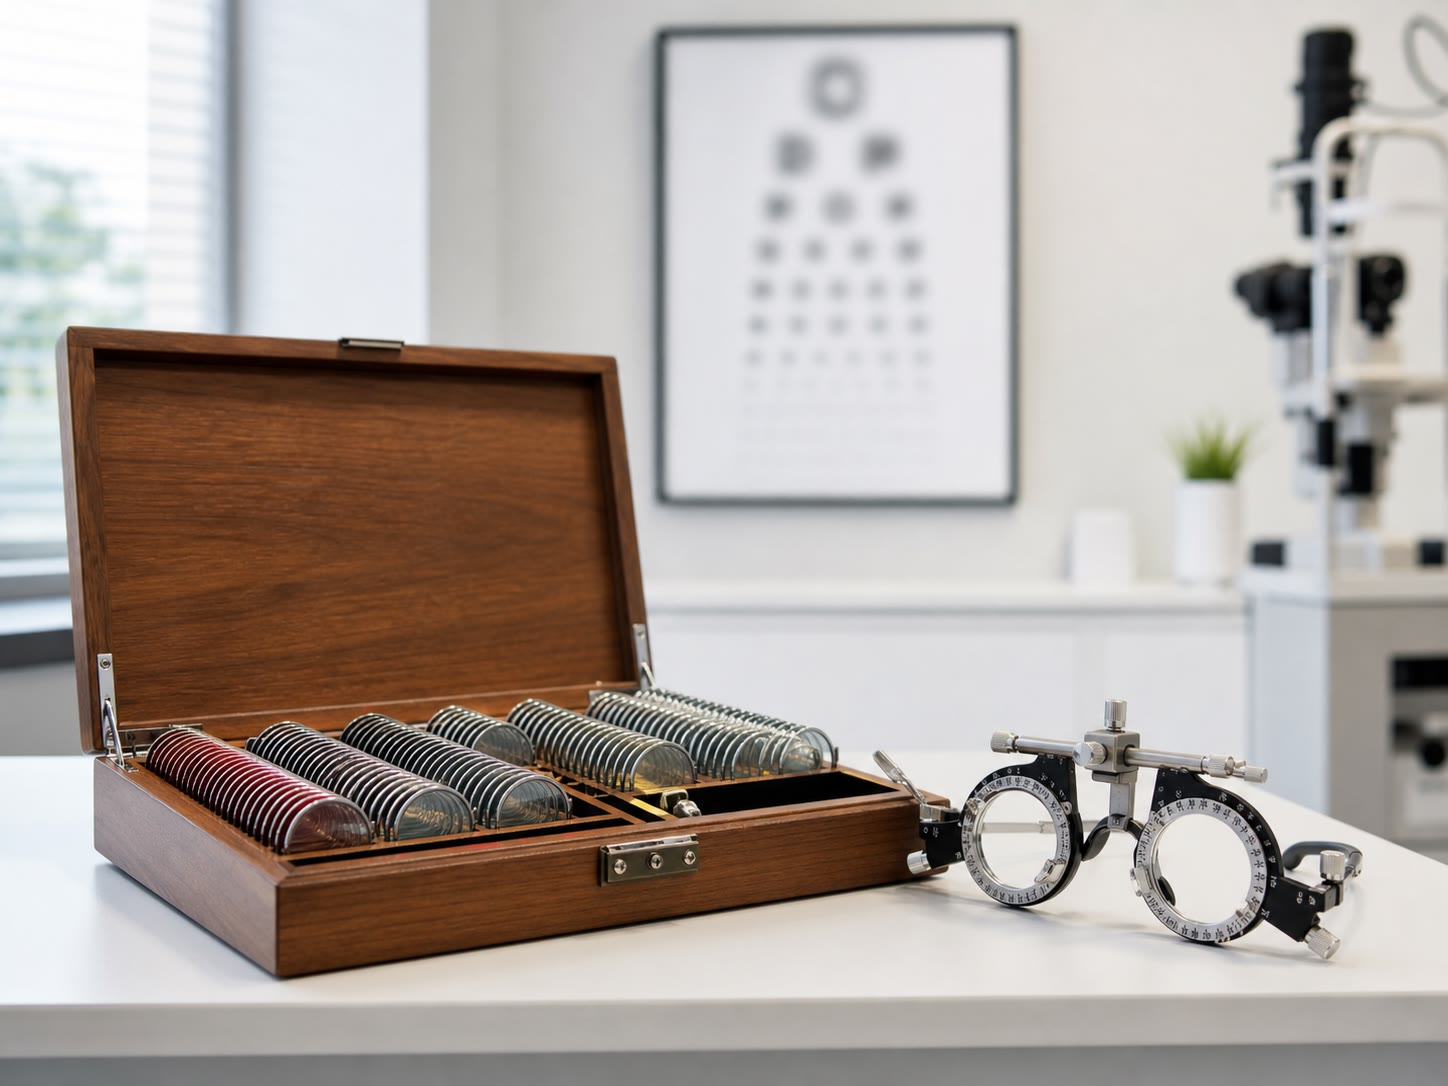
\includegraphics[width=0.50\linewidth]{images/book3/ai/b3-04-eye-chart-trial-frame.jpg}

{\small Boîte de verres d'essai et monture d'essai d'un opticien~: une \omterm{def:b1:mirrors-thin-lenses:lens}{lentille convergente} ou divergente de la bonne \omterm{def:b1:mirrors-thin-lenses:lens}{vergence}, placée devant l'\omterm{def:b1:optical-instruments:eye}{œil}, ramène son \omterm{def:b1:optical-instruments:punctum}{punctum remotum} à l'infini.}
\end{omfigure}

\section{Exercices}

\begin{exercise}[$\star$]\label{exo:b1:optical-instruments:1}
La \omterm{def:b1:optical-instruments:eye}{rétine} étant \qty{17}{mm} derrière le cristallin, calculer la \omterm{def:b1:mirrors-thin-lenses:lens}{vergence}
d'un \omterm{def:b1:optical-instruments:eye}{œil} normal qui regarde à l'infini, puis à \qty{25}{cm}~; en déduire
l'\omterm{def:b1:optical-instruments:punctum}{amplitude d'accommodation}. À quelles \omterm{def:b1:mirrors-thin-lenses:lens}{distances focales} cela
correspond-il~?
\end{exercise}

\begin{exercise}[$\star$]\label{exo:b1:optical-instruments:2}
Un \omterm{def:b1:optical-instruments:eye}{œil} myope a son \omterm{def:b1:optical-instruments:punctum}{punctum remotum} à \qty{40}{cm}. Quelle \omterm{def:b1:mirrors-thin-lenses:lens}{lentille} le
corrige (\omterm{def:b1:mirrors-thin-lenses:lens}{distance focale}, \omterm{def:b1:mirrors-thin-lenses:lens}{vergence})~? Un \omterm{def:b1:optical-instruments:eye}{œil} hypermétrope ne peut
accommoder sur rien de plus proche que \qty{1.0}{m}~: quelle \omterm{def:b1:mirrors-thin-lenses:lens}{lentille}
lui permet de lire à \qty{25}{cm}~?
\end{exercise}

\begin{exercise}[$\star$]\label{exo:b1:optical-instruments:3}
Une \omterm{def:b1:optical-instruments:G}{loupe} a $f' = \qty{4.0}{cm}$. Donner son \omterm{def:b1:optical-instruments:G}{grossissement}, la position
où tenir le timbre, et le \omterm{def:b1:optical-instruments:angular}{diamètre apparent} d'un détail de \qty{2}{mm}
à travers elle, comparé à celui vu à l'\omterm{def:b1:optical-instruments:eye}{œil} nu à \qty{25}{cm}.
\end{exercise}

\begin{exercise}[$\star$]\label{exo:b1:optical-instruments:4}
Une lunette a $f_1' = \qty{900}{mm}$. Calculer $G$ avec un \omterm{def:b1:optical-instruments:microscope}{oculaire} de
\qty{25}{mm} puis de \qty{9}{mm}, la longueur du tube dans chaque cas,
et le \omterm{def:b1:optical-instruments:angular}{diamètre apparent} de la Lune ($0.52^\circ$).
\end{exercise}

\begin{exercise}[$\star\star$]\label{exo:b1:optical-instruments:5}
\omterm{def:b1:optical-instruments:microscope}{Microscope}~: $f_1' = \qty{4.0}{mm}$, $f_2' = \qty{20}{mm}$,
$\Delta = \qty{160}{mm}$. Calculer $\gamma_1$, $G_2$, $G$, et la distance
objet--objectif. De combien faut-il déplacer le tube pour mettre au point
\qty{10}{\micro m} plus profond dans l'objet~?
\end{exercise}

\begin{exercise}[$\star\star$]\label{exo:b1:optical-instruments:6}
Deux phares sont distants de \qty{1.5}{m}. À partir de quelle distance
l'\omterm{def:b1:optical-instruments:eye}{œil} nu ($\epsilon = \qty{3e-4}{rad}$) cesse-t-il de les distinguer~?
Pour une lunette de $D = \qty{100}{mm}$~: calculer sa limite de
diffraction ($\lambda =
\qty{550}{nm}$), la distance à laquelle elle sépare les phares, et le
\omterm{def:b1:optical-instruments:G}{grossissement} $G_r$ au-delà duquel elle ne montre rien de nouveau.
\end{exercise}

\begin{exercise}[$\star\star$]\label{exo:b1:optical-instruments:7}
Un \omterm{def:b1:optical-instruments:microscope}{objectif} de \qty{50}{mm} à $f/2$~: quel est le diamètre de
l'ouverture~? Une scène est correctement exposée à $f/2$ en
$1/500$~\unit{s}~; quel temps de pose à $f/8$~? Qu'apporte la plus
petite ouverture~?
\end{exercise}

\begin{exercise}[$\star\star$]\label{exo:b1:optical-instruments:8}
Calculer la \omterm{prop:b1:optical-instruments:dof}{distance hyperfocale} d'un \omterm{def:b1:optical-instruments:microscope}{objectif} de \qty{35}{mm} à $f/11$
avec $c = \qty{0.03}{mm}$, et l'intervalle des distances nettes lorsqu'il
est mis au point sur $H$. Les photographes de rue préréglent ainsi~:
pourquoi~?
\end{exercise}

\begin{exercise}[$\star\star$]\label{exo:b1:optical-instruments:9}
Des jumelles «~$8\times30$~» ont $G = 8$ et $D = \qty{30}{mm}$. Calculer
le \omterm{prop:b1:optical-instruments:telescope}{cercle oculaire}~; toute la lumière est-elle utilisée par une pupille
nocturne de \qty{7}{mm}~? Et pour des «~$7\times50$~»~? Quelle paire
vaut mieux au crépuscule, et pourquoi des «~$20\times30$~» sont-elles un
mauvais choix~?
\end{exercise}

\begin{exercise}[$\star\star\star$]\label{exo:b1:optical-instruments:10}
Le \omterm{def:b1:optical-instruments:punctum}{punctum remotum} d'un myope est à \qty{25}{cm} de l'\omterm{def:b1:optical-instruments:eye}{œil}. Calculer la
\omterm{def:b1:mirrors-thin-lenses:lens}{vergence} de la \omterm{def:b1:mirrors-thin-lenses:lens}{lentille} de contact qui le corrige, puis celle de verres
de lunettes portés \qty{15}{mm} devant l'\omterm{def:b1:optical-instruments:eye}{œil}. Quelle correction est la
plus forte, et pourquoi les deux diffèrent-elles~?
\end{exercise}

\begin{exercise}[$\star\star\star$]\label{exo:b1:optical-instruments:11}
Lunette de Galilée~: $f_1' = \qty{30}{cm}$, $f_2' = \qty{-10}{cm}$.
Trouver l'écart des \omterm{def:b1:mirrors-thin-lenses:lens}{lentilles} pour un \omterm{prop:b1:mirrors-thin-lenses:doublet}{système afocal}, $G$, et
l'orientation de l'image. Situer le \omterm{prop:b1:optical-instruments:telescope}{cercle oculaire} et expliquer
pourquoi le champ est étroit.
\end{exercise}

\begin{exercise}[$\star\star\star$]\label{exo:b1:optical-instruments:12}
Une lunette de \qty{200}{mm} et une pupille de \qty{7}{mm}. De quel
facteur la lumière reçue d'une étoile est-elle augmentée~? Les
astronomes classent les éclats en magnitudes,
$m_2 - m_1 = 2.5\log_{10}(F_1/F_2)$~; l'\omterm{def:b1:optical-instruments:eye}{œil} atteint la magnitude $6$~:
quelle magnitude limite la lunette donne-t-elle~? Combien de fois plus
loin une même lampe peut-elle être vue~?
\end{exercise}

\begin{omfigure}
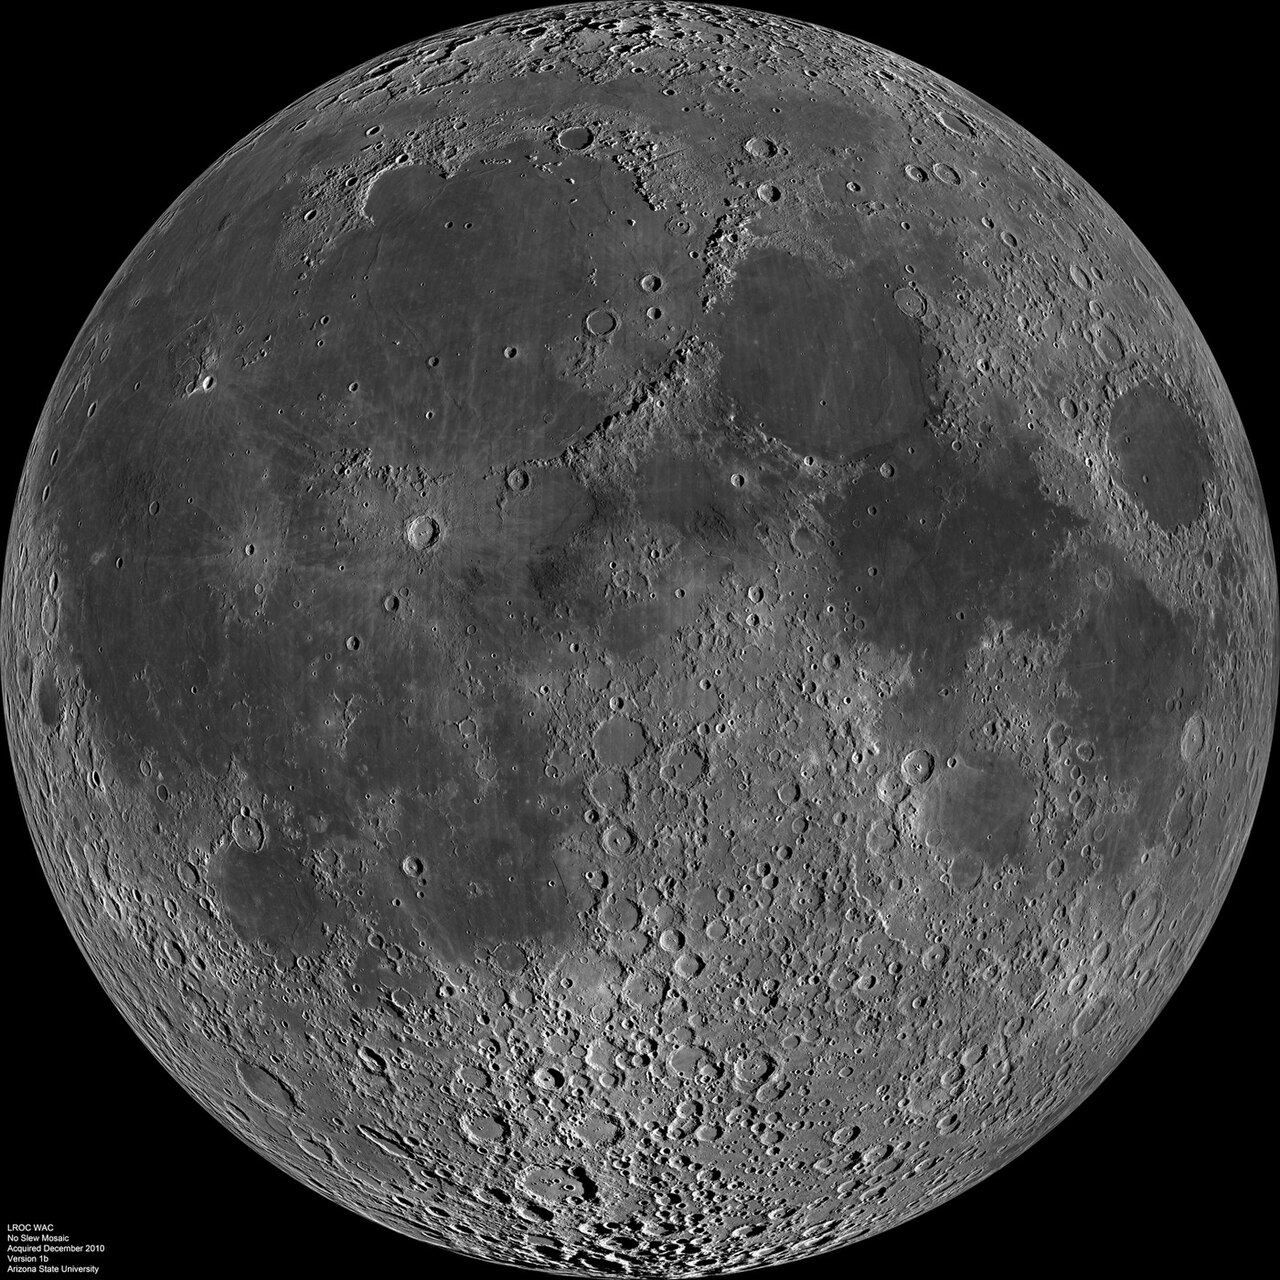
\includegraphics[width=0.40\linewidth]{images/book3/moon-nearside-lro.jpg}

{\small La face visible de la Lune (Lunar Reconnaissance Orbiter, NASA)~: la cible de la lunette du problème du week-end, \qty{3476}{km} de diamètre à \qty{384000}{km}.}
\end{omfigure}

\section{Problème~: concevoir une lunette pour la Lune}

\begin{problem}[{Problème du week-end --- une lunette de 150 millimètres
sur une pelouse~: choisir les oculaires, placer l'œil, compter la
lumière, et découvrir le plus petit cratère qu'elle sait montrer}]
\label{pb:b1:optical-instruments:1}
L'\omterm{def:b1:optical-instruments:microscope}{objectif} est une \omterm{def:b1:mirrors-thin-lenses:lens}{lentille convergente} $L_1$ de \omterm{def:b1:mirrors-thin-lenses:lens}{distance focale}
$f_1' = \qty{1200}{mm}$ et de diamètre $D = \qty{150}{mm}$~; on dispose
d'\omterm{def:b1:optical-instruments:microscope}{oculaires} $L_2$ de \omterm{def:b1:mirrors-thin-lenses:lens}{distances focales} \qty{25}{mm} et \qty{6}{mm}. La
Lune est à \qty{3.84e5}{km} et vue sous $0.52^\circ$~; la pupille
nocturne de l'\omterm{def:b1:optical-instruments:eye}{œil} vaut \qty{7}{mm}, sa résolution
$\epsilon = \qty{3.0e-4}{rad}$~; $\lambda = \qty{550}{nm}$.

\medskip
\noindent\textbf{Partie I --- Le montage afocal.}
\begin{enumerate}
  \item Où faut-il placer l'\omterm{def:b1:optical-instruments:microscope}{oculaire} pour qu'une étoile soit vue sans
        \omterm{def:b1:optical-instruments:eye}{accommodation}~? Donner la distance objectif--oculaire pour
        chaque \omterm{def:b1:optical-instruments:microscope}{oculaire}.
  \item Vérifier, en appliquant la \omterm{thm:b1:mirrors-thin-lenses:lensconj}{relation de Descartes} à chaque
        \omterm{def:b1:mirrors-thin-lenses:lens}{lentille} tour à tour, qu'un point à l'infini sur l'axe est imagé
        à l'infini.
  \item Montrer qu'un faisceau venu d'une étoile située à l'angle
        $\alpha$ de l'axe émerge en faisceau parallèle sous l'angle
        $\alpha' = -(f_1'/f_2')\alpha$.
  \item Calculer $G$ pour chaque \omterm{def:b1:optical-instruments:microscope}{oculaire} et le \omterm{def:b1:optical-instruments:angular}{diamètre apparent} de la
        Lune à travers chacun.
  \item L'image est renversée. Pourquoi est-ce acceptable ici, et
        qu'ajouterait une lunette terrestre~?
  \item Où se trouve l'image intermédiaire réelle de la Lune, et quel
        est son diamètre~? (On peut l'y photographier.)
\end{enumerate}

\medskip
\noindent\textbf{Partie II --- Où placer l'\omterm{def:b1:optical-instruments:eye}{œil}.}
\begin{enumerate}[resume]
  \item Montrer que l'\omterm{def:b1:optical-instruments:microscope}{oculaire} forme du bord de l'\omterm{def:b1:optical-instruments:microscope}{objectif} une \omterm{def:b1:mirrors-thin-lenses:image}{image
        réelle} en $\overline{O_2P'} = f_2'(f_1' + f_2')/f_1'$ derrière
        lui, de diamètre $D/\abs G$ (le \omterm{prop:b1:optical-instruments:telescope}{cercle oculaire}).
  \item Calculer la position et le diamètre du \omterm{prop:b1:optical-instruments:telescope}{cercle oculaire} pour
        chaque \omterm{def:b1:optical-instruments:microscope}{oculaire}.
  \item Pourquoi la pupille de l'\omterm{def:b1:optical-instruments:eye}{œil} doit-elle être placée sur le \omterm{prop:b1:optical-instruments:telescope}{cercle
        oculaire}~? Qu'advient-il du champ si on la place plus loin~?
  \item Pour que la lumière d'une étoile soit intégralement utilisée, le
        \omterm{prop:b1:optical-instruments:telescope}{cercle oculaire} ne doit pas dépasser la pupille de l'\omterm{def:b1:optical-instruments:eye}{œil}~: en
        déduire le \omterm{def:b1:optical-instruments:G}{grossissement} utile minimal de cette lunette la nuit.
\end{enumerate}

\medskip
\noindent\textbf{Partie III --- La résolution.}
\begin{enumerate}[resume]
  \item Calculer la limite de diffraction $\theta_{\min} = 1.22\lambda/D$
        en radians et en secondes d'arc.
  \item À quel plus petit cratère cet angle correspond-il sur la Lune~?
        Et pour l'\omterm{def:b1:optical-instruments:eye}{œil} nu~?
  \item Définir et calculer le \omterm{def:b1:optical-instruments:G}{grossissement} résolvant $G_r =
        \epsilon/\theta_{\min}$. Quel \omterm{def:b1:optical-instruments:microscope}{oculaire} en est le plus proche~?
  \item Avec l'\omterm{def:b1:optical-instruments:microscope}{oculaire} de \qty{6}{mm}, l'image paraît plus floue et
        plus terne qu'avec celui de \qty{25}{mm}. Expliquer les deux
        effets.
  \item La turbulence atmosphérique étale les images d'étoiles sur
        environ $1''$. Pour quels diamètres d'\omterm{def:b1:optical-instruments:microscope}{objectif} la limite de
        Rayleigh cesse-t-elle de compter depuis le sol, et qu'apporte
        encore un $D$ plus grand~?
\end{enumerate}

\medskip
\noindent\textbf{Partie IV --- La lumière.}
\begin{enumerate}[resume]
  \item De quel facteur l'\omterm{def:b1:optical-instruments:microscope}{objectif} recueille-t-il plus de lumière que la
        pupille nocturne~?
  \item Convertir en magnitudes ($\Delta m = 2.5\log_{10}$ du rapport)~;
        si l'\omterm{def:b1:optical-instruments:eye}{œil} atteint la magnitude $6$, quelle magnitude la lunette
        atteint-elle~?
  \item La pleine Lune délivre au sol un éclairement d'environ
        \qty{2e-3}{W/m^2}. Quelle puissance entre dans l'\omterm{def:b1:optical-instruments:microscope}{objectif}, et
        comment se répartit-elle sur la \omterm{def:b1:optical-instruments:eye}{rétine} par rapport à
        l'observation à l'\omterm{def:b1:optical-instruments:eye}{œil} nu (même raisonnement de puissance par
        unité d'angle solide~: comparer la luminance à travers les deux
        \omterm{def:b1:optical-instruments:microscope}{oculaires})~?
  \item Pourquoi une lunette ne rend-elle pas la surface de la Lune plus
        lumineuse par unité d'aire que l'\omterm{def:b1:optical-instruments:eye}{œil} nu, alors qu'elle rend bien
        les étoiles plus brillantes~?
\end{enumerate}

\medskip
\noindent\textbf{Partie V --- Le champ de vision.}
L'\omterm{def:b1:optical-instruments:microscope}{oculaire} porte, dans son plan focal, un diaphragme de champ circulaire
de diamètre \qty{20}{mm} (\omterm{def:b1:optical-instruments:microscope}{oculaire} de \qty{25}{mm}) ou \qty{5}{mm}
(\omterm{def:b1:optical-instruments:microscope}{oculaire} de \qty{6}{mm}).
\begin{enumerate}[resume]
  \item Montrer que le champ réel vaut $2\arctan(\phi/2f_1')
        \approx \phi/f_1'$ pour un diaphragme de diamètre $\phi$.
  \item Le calculer pour les deux \omterm{def:b1:optical-instruments:microscope}{oculaires} et dire si la Lune entière
        tient dans le champ.
  \item Calculer le champ apparent (l'angle sous lequel l'\omterm{def:b1:optical-instruments:eye}{œil} voit le
        diaphragme à travers l'\omterm{def:b1:optical-instruments:microscope}{oculaire}) pour les deux.
  \item La Terre tourne de $15''$ par seconde de temps~: combien de
        temps la Lune met-elle à traverser le champ de chaque \omterm{def:b1:optical-instruments:microscope}{oculaire}
        sans suivi~?
  \item Récapituler la conception~: quel \omterm{def:b1:optical-instruments:microscope}{oculaire} pour la Lune entière,
        lequel pour les cratères, et la taille du plus petit cratère que
        l'instrument sait révéler --- son unique nombre.
  \item Le même \omterm{def:b1:optical-instruments:microscope}{objectif} est remplacé par un \omterm{def:b1:mirrors-thin-lenses:mirror}{miroir concave} de
        \qty{150}{mm} et de même \omterm{def:b1:mirrors-thin-lenses:lens}{distance focale}. Lesquels des résultats
        précédents changent~?
\end{enumerate}
\end{problem}
